\title{Rokkoチュートリアル}

\begin{document}

\lstset{language={sh},showspaces=false,rulecolor=\color[cmyk]{0, 0.29,0.84,0}}

\begin{frame}
  \titlepage
  \noindent {\footnotesize 本資料のソースは\url{https://github.com/cmsi/rokko-tutorial}にて公開中}
\end{frame}

%% \section*{Outline}
%% \begin{frame}
%%   \tableofcontents
%% \end{frame}

\section{チュートリアルの概要}

\begin{frame}{Rokkoチュートリアル スタッフ}
  \begin{itemize}
  \item 講師
    \setlength{\itemsep}{1em}
    \begin{itemize}
      \setlength{\itemsep}{1em}
    \item 藤堂眞治 (東大院理) \ \href{mailto:wistaria@phys.s.u-tokyo.ac.jp}{wistaria@phys.s.u-tokyo.ac.jp}
    \item 五十嵐 亮 (東大物性研) \ \href{mailto:rigarash@issp.u-tokyo.ac.jp}{rigarash@issp.u-tokyo.ac.jp}
    \item 本山裕一 (東大院工 $\Rightarrow $ 物性研) \ \href{mailto:yomichi@looper.u-tokyo.ac.jp}{yomichi@looper.t.u-tokyo.ac.jp}
    \end{itemize}
  \item 主催
    \begin{itemize}
    \item CMSI: 計算物質科学イニシアティブ \url{http://cms-initiative.jp/}
    \end{itemize}
  \end{itemize}
\end{frame}

\begin{frame}
  \frametitle{チュートリアルの流れ}
  \begin{itemize}
    %\setlength{\itemsep}{1em}
  \item 座学: 既存の固有値問題の解法・固有値ソルバ/線形計算ライブラリ
  \item 座学: Rokkoの概要と内部構造
  \item 実習: サンプルの実行
  \item 実習: アプリケーションからのRokkoの利用
  \item 座学/実習: Rokkoのインストール
  \item (付録: ALPS/Baristaパッケージ)
  \item (付録: MateriAppsとMateriApps LIVE!)
  \end{itemize}
\end{frame}

\begin{frame}
  \frametitle{ネットワーク設定}
  \begin{itemize}
    \setlength{\itemsep}{1em}
  \item LAN接続 (無線 or 有線)
  \item 講習会資料ダウンロード
  \item 実習用ワークステーションのアカウント登録
  \item 実習用ワークステーションへのログイン確認
  \end{itemize}
\end{frame}

\section{固有値問題の解法・固有値ソルバ/線形計算ライブラリ}

\begin{frame}
  \frametitle{固有値問題の解法・固有値ソルバ/線形計算ライブラリ}
  \begin{itemize}
    \setlength{\itemsep}{1em}
  \item 行列の対角化
  \item 固有値問題の解法
  \item 既存の固有値ソルバ/線形計算ライブラリ
  \end{itemize}
\end{frame}

\begin{frame}
  \frametitle{行列の対角化}
  \begin{itemize}
    %\setlength{\itemsep}{1em}
  \item 行列の種類
    \begin{itemize}
    \item 実対称行列, 実非対称行列, エルミート行列, 非エルミート行列
    \end{itemize}
  \item 行列の表示
    \begin{itemize}
      \item 密行列, CRS形式, MatFree形式 (それぞれTITPACK2の「小規模」, 
        「中規模」, 「大規模」に対応)
    \end{itemize}
  \item 必要な固有値
    \begin{itemize}
      \item 全て, 絶対値の大きな(小さな)順にいくつか, ある範囲内
    \end{itemize}
  \item 固有ベクトル
    \begin{itemize}
      \item 要/不要
    \end{itemize}
  \end{itemize}
\end{frame}

\begin{frame}
  \frametitle{用語の定義}
  \begin{itemize}
    %\setlength{\itemsep}{1em}
  \item 固有値問題の解法(Eigenvalue algorithm)
    \begin{itemize}
      \item 固有値問題を解くためのアルゴリズム
    \end{itemize}
  \item 固有値ソルバ(Eigensolver, Eigenvalue problem solver)
    \begin{itemize}
      \item 固有値解法の実装
    \end{itemize}
  \item 固有値ソルバライブラリ(Eigensolver LIbrary)
    \begin{itemize}
      \item 固有値ソルバのみを含むライブラリ
    \end{itemize}
  \item 線形計算ライブラリ(Linear Algebra Library)
    \begin{itemize}
      \item 固有値ソルバや他の線形計算ソルバの集合体
    \end{itemize}
  \item 厳密対角化パッケージ(Exact diaognalization package)
    \begin{itemize}
      \item 量子格子模型のハミルトニアンの固有値問題を扱うソフトウェア
    \end{itemize}
  \end{itemize}
\end{frame}

\begin{frame}
  \frametitle{固有値問題の解法(一部)}
  \begin{itemize}
    %\setlength{\itemsep}{1em}
  \item 三重対角行列に対する固有値問題の解法
    \begin{itemize}
      \item 二分法, QR法, MR3, 分割統治法+QR法
    \end{itemize}
  \item 密行列の直接対角化
    \begin{itemize}
      \item Jacobi法
    \end{itemize}
  \item 密行列の三重対角化
    \begin{itemize}
      \item Householder法
    \end{itemize}
  \item 疎行列の直接対角化
    \begin{itemize}
      \item べき乗法, 逆べき乗法, レイリー商反復法, Jacobi-Davidson法, LOBPCG, Krylov-Schur法
    \end{itemize}
  \item 疎行列の三重対角化
    \begin{itemize}
      \item Lanczos法, Arnoldi法, リスタート付きLanczos法(Restart Lanczos), Thick-restart Lanczos
    \end{itemize}
  \item その他の方法
    \begin{itemize}
      \item Sakurai-Sugiura法
    \end{itemize}
  \end{itemize}
\end{frame}

\begin{frame}
  \frametitle{固有値問題の解法}
  \begin{center}
    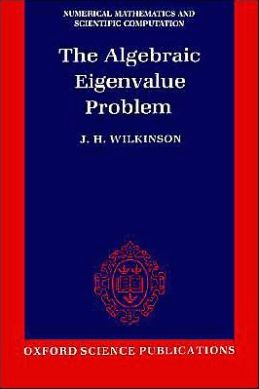
\includegraphics[height=0.6\textheight]{figure/AlgebraicEigenvalue.jpg} \ \
    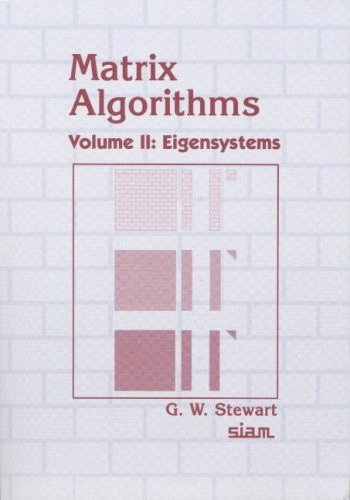
\includegraphics[height=0.6\textheight]{figure/MatrixAlgorithms.jpg} \ \
    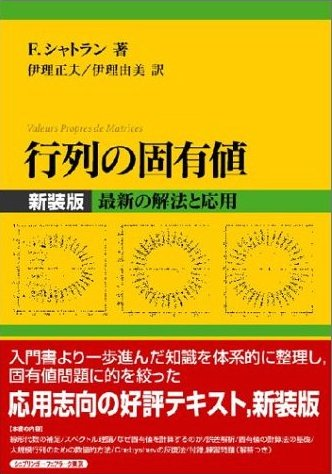
\includegraphics[height=0.6\textheight]{figure/book.jpg}
  \end{center}
\end{frame}

\begin{frame}
  \frametitle{既存の固有値ソルバライブラリ(一部)}
  \begin{itemize}
    %\setlength{\itemsep}{1em}
  \item Anasazi: 反復法ソルバ中心
    \begin{itemize}
      \item Krylov-Schur, Jacobi-Davidson, XXX-Davidson, LOBPCG, Implicit Riemann Trust Region Method
    \end{itemize}
  \item EigenExa: 密行列ソルバ
    \begin{itemize}
      \item Householder (3重対角化, 5重対角化)+分割統治法+QR
    \end{itemize}
  \item ELPA
    \begin{itemize}
      \item Householder+分割統治法+QR
    \end{itemize}
  \item IETL: ALPSに含まれる反復法ソルバ
    \begin{itemize}
      \item Lanczos, 他
    \end{itemize}
  \end{itemize}
\end{frame}

\begin{frame}
  \frametitle{既存の線形計算ライブラリ(一部)}
  \begin{itemize}
    %\setlength{\itemsep}{1em}
  \item Apple VecLib: LAPACK
  \item ARPACK
    \begin{itemize}
      \item Implicit Restarted Lanczos
    \end{itemize}
  \item BLOPEX
  \item Eigen3: MPI並列(プロセス数が平方数の場合のみ)
    \begin{itemize}
      \item Householder+QR
    \end{itemize}
  \item Elemental
    \begin{itemize}
      \item Householder+MR3
    \end{itemize}
  \item Fujitsu SSLII: LAPACK, ScaLAPACK(の一部), 他
  \item Intel MKL: LAPACK, ScaLAPACK
  \end{itemize}
\end{frame}

\begin{frame}
  \frametitle{既存の線形計算ライブラリ(一部)}
  \begin{itemize}
    %\setlength{\itemsep}{1em}
  \item Netlib LAPACK: LAPACKのリファレンス実装
    \begin{itemize}
      \item Householder+QR, Householder+分割統治法+QR, Householder+二分法, Householder+MR3
    \end{itemize}
  \item Netlib ScaLAPACK: ScaLAPACKのリファレンス実装
    \begin{itemize}
      \item Householder+QR, Householder+分割統治法+QR, Householder+二分法, Householder+MR3
    \end{itemize}
  \item SLEPc: 反復法ソルバ中心, ビルド時に逐次かMPI並列かを選ぶ必要あり
    \begin{itemize}
      \item Krylov-Schur, Generalized Davidson, Jacobi-Davidson, Rayleigh Quotient Conjugate Gradient, Contour integral Sakurai-Sugiura, Power method, Subspace Itertation, Arnoldi (explicit restart), Lanczos (explicit restart) \\
    \end{itemize}
  \item Xabclib (ppOpen AT)
  \end{itemize}
\end{frame}

\begin{frame}
  \frametitle{おすすめ順}
  \begin{itemize}
    %\setlength{\itemsep}{1em}
  \item 密行列・逐次 \\
    LAPACK (のベンダ実装) $>$ Eigen3
  \item 密行列・MPI並列 \\
    EigenExa $>$ ELPA $>$ ScaLAPACK (のベンダ実装) $>$ Elemental
  \item 疎行列・逐次 \\
    Anasazi
  \item 疎行列・MPI並列 \\
    Anasazi $>$ SLEPc \\
  \item ハイブリッド並列対応のソルバも増えてきた
  \item 並列版をユーザが実装・最適化するのはもはや不可能
  \item オープンソースの最新並列固有値ソルバを積極的に活用すべき
  \end{itemize}
\end{frame}

\begin{frame}{EigenExaによる超巨大密行列の対角化}
  \begin{center}
    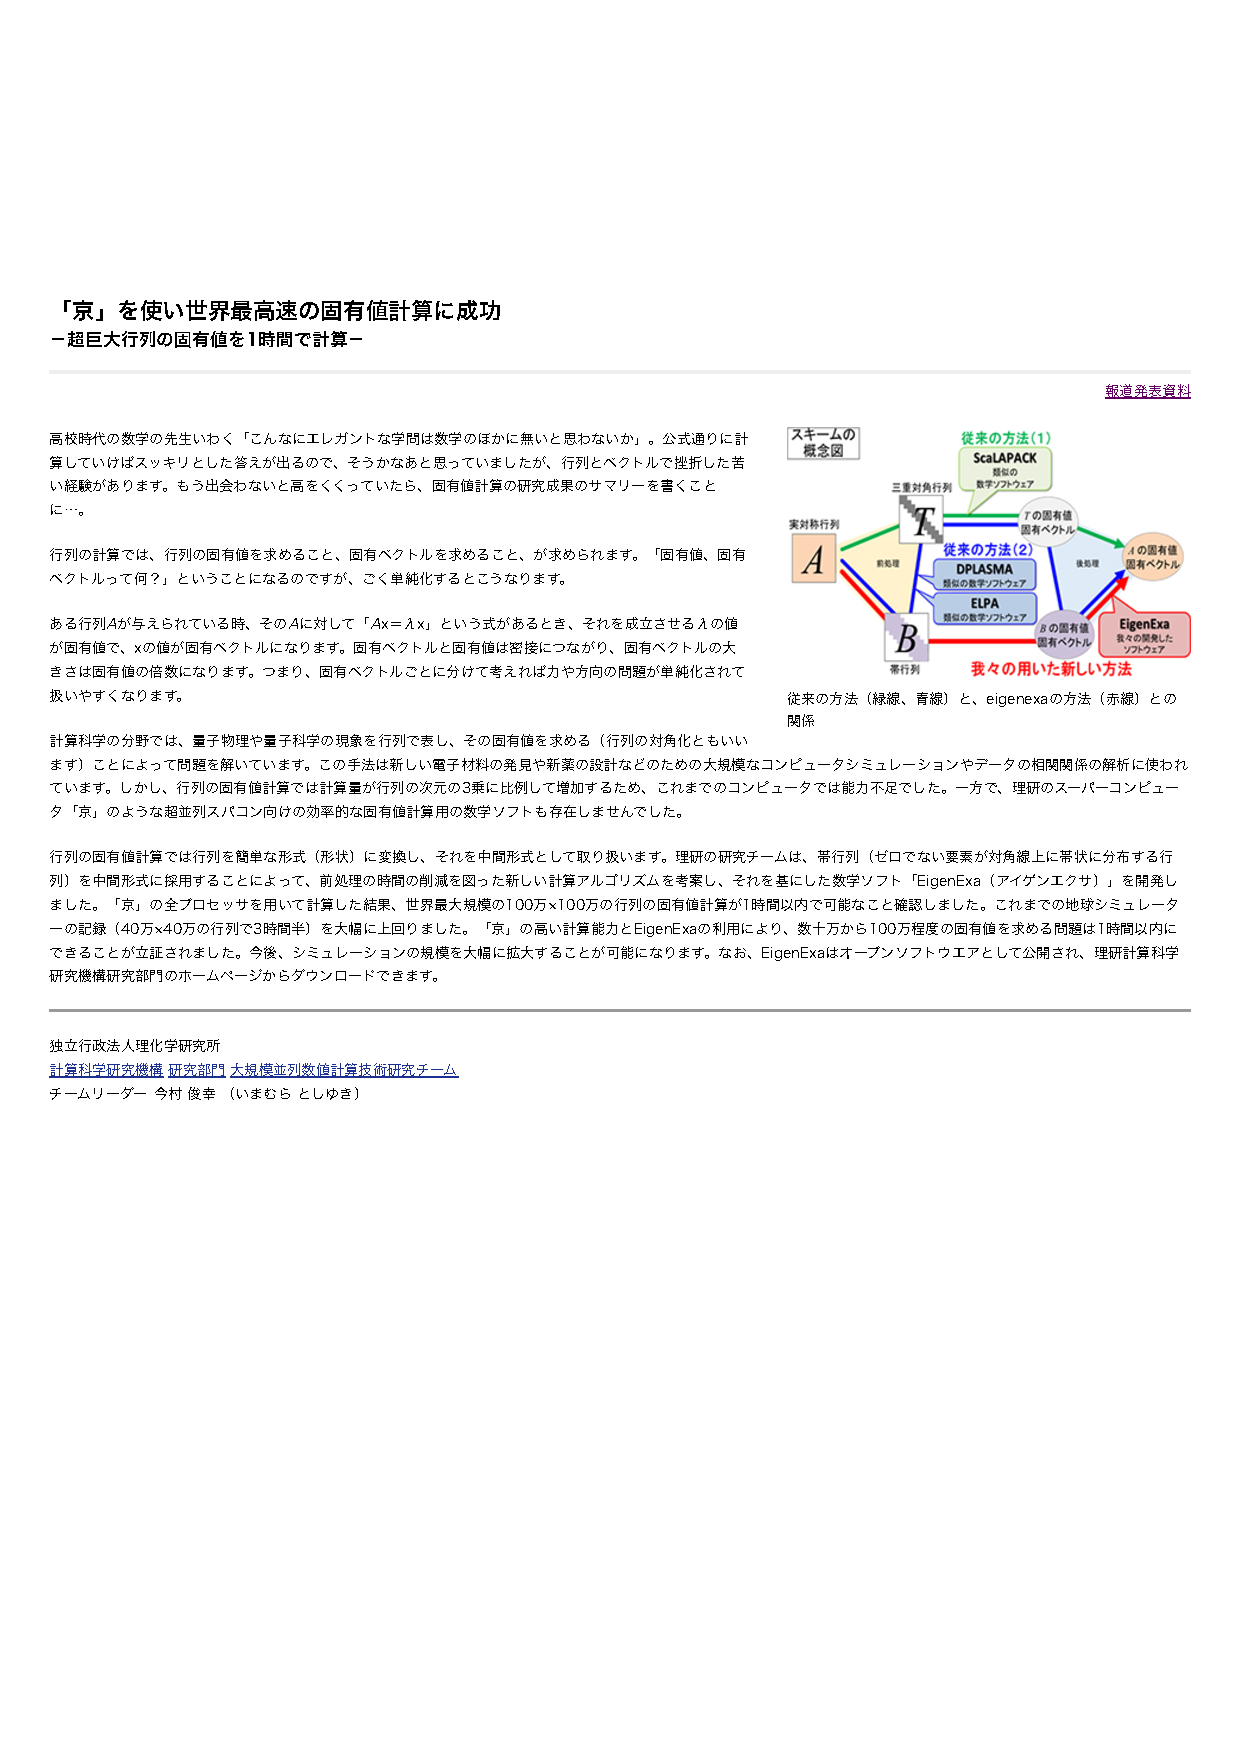
\includegraphics[height=0.8\textheight]{figure/eigenexa.pdf}
  \end{center}
\end{frame}

\begin{frame}
  \frametitle{最新の固有値ソルバ}
  \begin{itemize}
    \setlength{\itemsep}{1em}
  \item ハイブリッド並列(MPI+OpenMP)対応のソルバも増えてきた
  \item 超並列環境に対応した並列ソルバを一般ユーザが実装・最適化するの
    はもはや不可能
  \item オープンソースの最新並列固有値ソルバを積極的に活用すべき
  \end{itemize}
\end{frame}

\begin{frame}
  \frametitle{厳密対角化パッケージの状況}
  \begin{itemize}
    \setlength{\itemsep}{1em}
  \item ALPS: LAPACK, IETLを利用
  \item KOBEPACK: 独自の固有値ソルバを実装
  \item SPINPACK: LAPACKを利用
  \item TITPACK2: 独自の固有値ソルバを実装 \\
  \item 逐次 or スレッド並列のみ、MPI並列なし
  \item 最新の超並列スパコン環境を活かしきれていない
  \end{itemize}
\end{frame}

\begin{frame}
  \frametitle{固有値解法とソルバ}
  \begin{itemize}
    \setlength{\itemsep}{1em}
    \item GitHub Wikiに, 固有値問題の解法, 固有値ソルバ, 固有値ソルバ/線形計算ライブラリ, 厳密対角化パッケージに関する辞書を作成中
      \begin{itemize}
        \item 固有値解法とソルバ: \url{https://github.com/t-sakashita/rokko/wiki/EigenvalueAlgorithms}
      \end{itemize}
    \item ボランティア募集中!
  \end{itemize}
\end{frame}
        
\section{Rokkoの概要と内部構造}

\begin{frame}
  \frametitle{Rokkoの概要と内部構造}
  \begin{itemize}
    \setlength{\itemsep}{1em}
  \item 既存のライブラリの問題点
  \item Rokkoの概要
  \item 並列ソルバの基本概念
  \item Rokkoの内部構造
  \end{itemize}
\end{frame}

\begin{frame}
  \frametitle{既存のライブラリの問題点}
  \begin{itemize}
    %\setlength{\itemsep}{1em}
  \item ソルバ毎に異なるデザイン
  \item インストール方法もライブラリ毎に異なる
  \item ドキュメントが不十分な場合も多い
  \item コンピュータのアーキテクチャ毎に異なるコンパイル・リンクオプションが必要
  \item C++/C/Fortran相互リンクの問題
  \item ライブラリ間の依存関係が複雑
  \item 実際に試す前に大まかな性能比較が欲しい
  \end{itemize}
\end{frame}

\begin{frame}
  \frametitle{ライブラリ間の依存関係(一部)}
  \begin{center}
    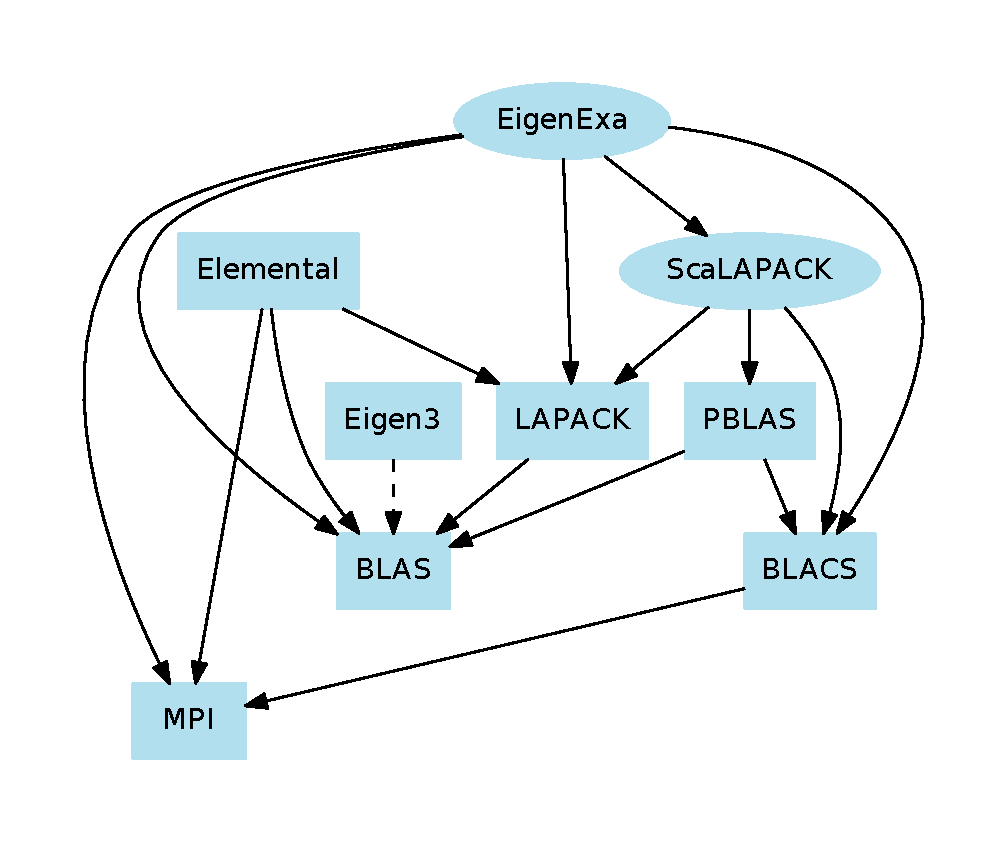
\includegraphics[height=0.8\textheight]{figure/library-dependence.pdf}
  \end{center}
\end{frame}

\begin{frame}
  \frametitle{Rokkoの開発者}
  \begin{itemize}
    \setlength{\itemsep}{1em}
  \item 坂下達哉 (東大物性研) \ \href{mailto:t-sakashita@issp.u-tokyo.ac.jp}{t-sakashita@issp.u-tokyo.ac.jp}
  \item 本山裕一 (東大院工 $\Rightarrow $ 物性研) \ \href{mailto:yomichi@looper.u-tokyo.ac.jp}{yomichi@looper.t.u-tokyo.ac.jp}
  \item 五十嵐 亮 (東大物性研) \ \href{mailto:rigarash@issp.u-tokyo.ac.jp}{rigarash@issp.u-tokyo.ac.jp}
  \item 大久保 毅 (東大物性研) \ \href{mailto:t-okubo@issp.u-tokyo.ac.jp}{t-okubo@issp.u-tokyo.ac.jp}
  \item 藤堂眞治 (東大院理/東大物性研) \ \href{mailto:wistaria@phys.s.u-tokyo.ac.jp}{wistaria@phys.s.u-tokyo.ac.jp}
  \end{itemize}
\end{frame}

\begin{frame}
  \frametitle{Rokkoの概要}
  \begin{itemize}
    %\setlength{\itemsep}{1em}
  \item 使用言語
    \begin{itemize}
      %\setlength{\itemsep}{1em}
    \item コア部分: C++
    \item 言語バインディング: C, Fortran90
    \item ベンチマークスクリプト: Python
    \end{itemize}
  \item ライセンス
    \begin{itemize}
      %\setlength{\itemsep}{1em}
    \item Boostライセンス (ほぼ自由に使える)
    \end{itemize}
  \item ソースコード
    \begin{itemize}
      %\setlength{\itemsep}{1em}
    \item GitHubで公開
    \item \url{https://github.com/t-sakashita/rokko}
    \end{itemize}
  \end{itemize}
\end{frame}

\begin{frame}
  \frametitle{Rokkoの設計方針}
  \begin{itemize}
    %\setlength{\itemsep}{1em}
  \item 共通のベクトルや行列クラス
  \item ソルバの違いをラッパーで吸収
    \begin{itemize}
      %\setlength{\itemsep}{1em}
    \item 個々のソルバに仕様変更があってもRokkoが吸収
    \end{itemize}
  \item 実行時にソルバを選択可能
  \item 仮想関数とテンプレートを組み合わせることで, オーバーヘッドの少ないラッパーを実装
  \item C++, C, Fortran90から使用可能に
  \end{itemize}
\end{frame}

\begin{frame}
  \frametitle{Rokkoの全体像}
  \begin{itemize}
    %\setlength{\itemsep}{1em}
  \item 固有値ソルバ/線形演算ライブラリのインストールスクリプト
  \item 共通基本クラス(分散行列, プロセスグリッド他)
  \item 固有値ソルバラッパー(C++)
  \item 固有値ソルバ・ファクトリ(C++)
  \item C/Fortranラッパー
  \item テスト・サンプルプログラム
  \item ベンチマークスクリプト
  \end{itemize}
\end{frame}

\begin{frame}
  \frametitle{Rokko Software Stack}
  \begin{center}
    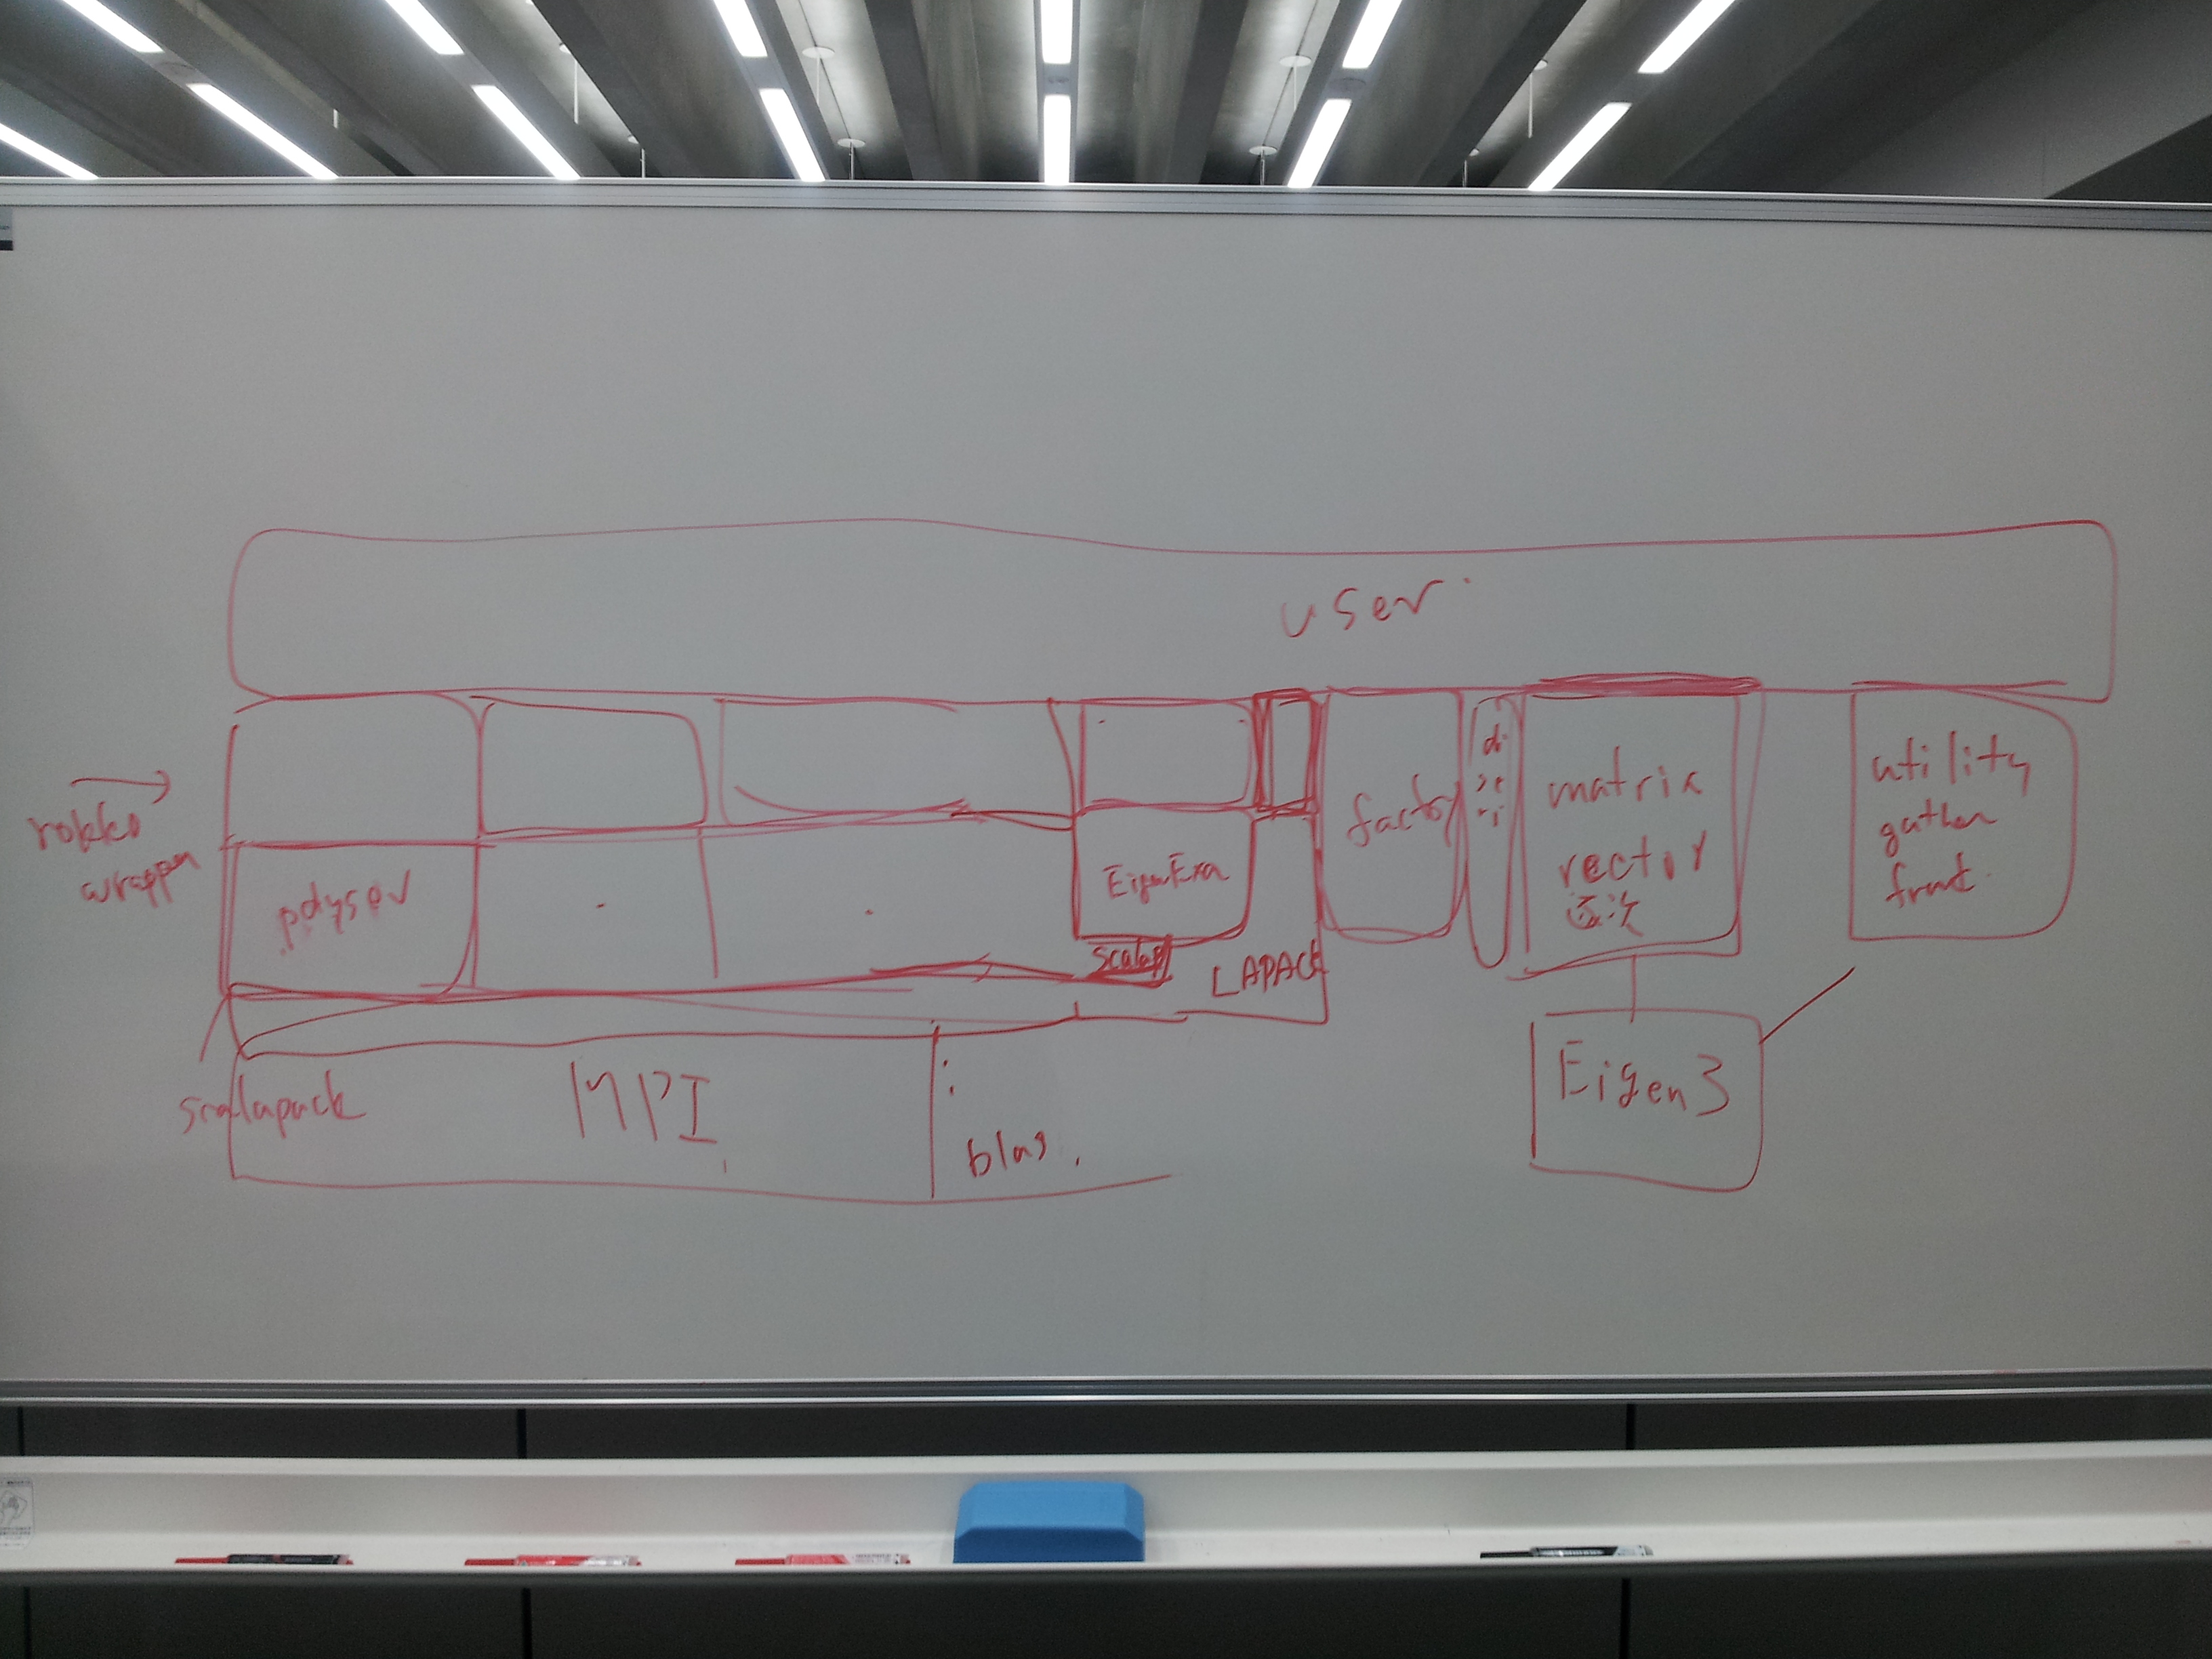
\includegraphics[height=0.8\textheight]{figure/rokko-software-stack.jpg}
  \end{center}
\end{frame}

\section{並列ソルバの基本概念}

\begin{frame}
  \frametitle{プロセスグリッド}
  \begin{itemize}
    %\setlength{\itemsep}{1em}
  \item MPIプロセスの2次元割付けを指定
  \item Row-majorとcolumn-majorの二種類
  \item ほとんどの並列固有値ソルバは両方の種類をサポート \\
    (Elementalはcolumn-majorのみサポート)
  \end{itemize}
\end{frame}

\begin{frame}
  \frametitle{分散行列(Distributed Matrix)}
  \begin{itemize}
    %\setlength{\itemsep}{1em}
  \item ほとんどの並列固有値ソルバにおいて, 密行列は「2次元ブロック・サイクリック形式」でデータ分割される
  \item 4プロセスでの例
  \item ScaLAPACKとELPAは任意のブロックサイズをサポート
  \item EigenExaとElementalは$1 \times 1$ブロックサイズのみをサポート
  \end{itemize}
\end{frame}

\begin{frame}
  \frametitle{rokko::grid クラス}
  \begin{itemize}
    %\setlength{\itemsep}{1em}
  \item MPIプロセスの2次元割付けを指定
  \item Row-majorとcolumn-majorの二種類
  \item ほとんどの並列固有値ソルバは両方の種類をサポート \\
    (Elementalはcolumn-majorのみサポート)
  \end{itemize}
\end{frame}

\begin{frame}
  \frametitle{rokko::localized\_matrix クラステンプレート}
  \begin{itemize}
    %\setlength{\itemsep}{1em}
  \item ほとんどの並列固有値ソルバにおいて, 密行列は「2次元ブロック・サイクリック形式」でデータ分割される
  \item 4プロセスでの例
  \item ScaLAPACKとELPAは任意のブロックサイズをサポート
  \item EigenExaとElementalは$1 \times 1$ブロックサイズのみをサポート
  \end{itemize}
\end{frame}

\begin{frame}
  \frametitle{rokko::distributed\_matrix クラステンプレート}
  \begin{itemize}
    %\setlength{\itemsep}{1em}
  \item 
  \end{itemize}
\end{frame}

\begin{frame}
  \frametitle{分散行列の操作}
  \begin{itemize}
    %\setlength{\itemsep}{1em}
  \item 行列の掛け算, 転置, scatter/gather
  \end{itemize}
\end{frame}

\begin{frame}
  \frametitle{分散行列の生成}
  \begin{itemize}
    %\setlength{\itemsep}{1em}
  \item 要素毎に代入 (globalな添字)
  \item 要素毎に代入 (localな添字)
  \item 関数の値で行列を埋める
  \item 分散行列の scatter と gather
  \end{itemize}
\end{frame}

\section{サンプルの実行}
\section{アプリケーションからのRokkoの利用}

\section{Rokkoのインストール}

\begin{frame}
  \frametitle{インストール作業に必須のツールとライブラリ}
  \begin{itemize}
    \setlength{\itemsep}{1em}
  \item CMake: \url{http:www.cmake.org}
  \item Boost C++ Libraries: \url{http://www.boost.org}
  \item インストールスクリプト
  \item 主要なスパコンにインストール済み
  \end{itemize}
\end{frame}

\begin{frame}
  \frametitle{サードパーティーの固有値ソルバ/線形計算ライブラリのインストール}
  \begin{itemize}
    \setlength{\itemsep}{1em}
  \item Eigen3, LAPACK-e (LAPACKのCバインディング)は, Rokkoに同梱されている
  \item インストールスクリプト: EigenExa, ELPA, Elemental, SLEPc
  \item 対応アーキテクチャ: 京/FX10, x86スパコン・クラスタ(Intelコンパイラ/GCC), Mac OS X (GCC)
  \item 主要なスパコンにインストール済み
  \end{itemize}
\end{frame}

\begin{frame}
  \frametitle{Rokkoのインストール}
  \begin{itemize}
    %\setlength{\itemsep}{1em}
  \item ソースコードのダウンロード・展開
  \item CMake
  \item Make
  \item テスト
  \end{itemize}
\end{frame}


\section{ALPS/Baristaパッケージ}
\section{MateriAppsとMateriApps LIVE!}

\begin{frame}
  \frametitle{テスト}
  \begin{itemize}
    %\setlength{\itemsep}{1em}
  \item テスト
  \end{itemize}
\end{frame}

\end{document}
